\documentclass{ximera}

%\colorlet{penColor}{blue!50!black} % Color of a curve in a plot
%\colorlet{gridColor}{gray!50} % Color of grid in a plot
%\colorlet{background}{white} % Color of the page
\newcommand{\ddx}{\frac{d}{dx}}
\newcommand{\dydx}{\frac{dy}{dx}}
\newcommand{\dd}[2][]{\frac{d #1}{d #2}}


\outcome{What is net area and how is it different from total area?}
\outcome{How can Riemann sums be used to find exact area?}
\outcome{What are the properties of definite integrals and why do they make sense?}
\outcome{Approximate net area.}
\outcome{Compute definite integrals using limits of Riemann sums.}
\outcome{Compute definite integrals using geometry.}
\outcome{Compute definite integrals using the properties of integrals.}

\title{Definite integrals}

\begin{document}

\begin{abstract}
  Definite integrals compute signed area.
\end{abstract}

\maketitle

Definite integrals, often simply called integrals, compute signed area. 

\begin{definition}\index{integral}\index{definite integral}
The \textbf{definite integral}
\[
\int_a^b f(x) \d x
\]
computes the signed area in the region $[a,b]$ between $f(x)$ and the
$x$-axis. If the region is above the $x$-axis, then the area has
positive sign. If the region is below the $x$-axis, then the area has
negative sign.
\end{definition}




\begin{question}
Use common formulas for area to compute
\[
\int_0^3 x \d x.
\]
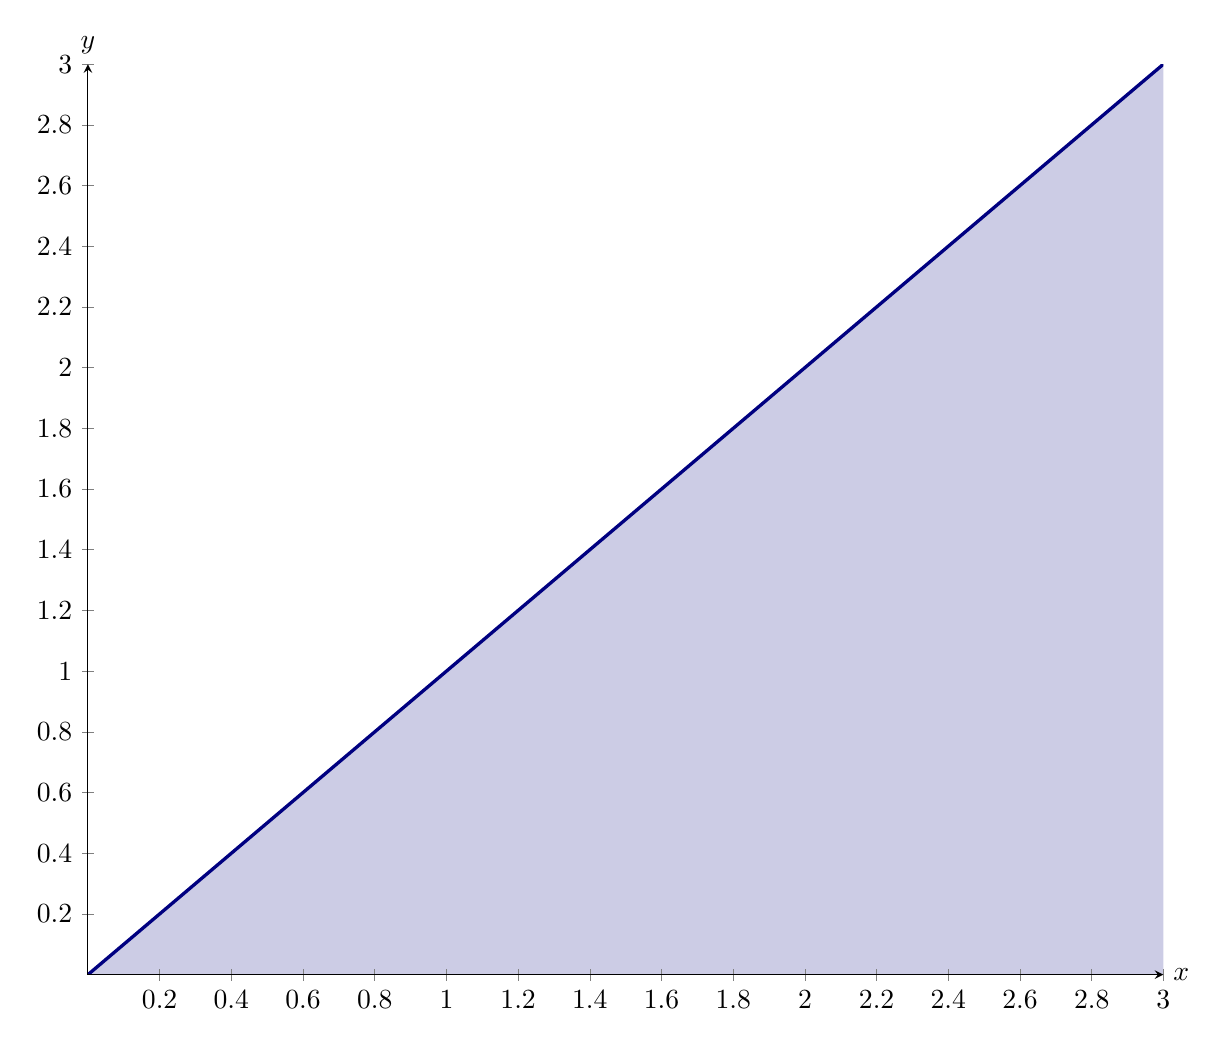
\begin{tikzpicture}
\colorlet{penColor}{blue!50!black}
\colorlet{fillp}{blue!50!black!20}
  \begin{axis}[
      width=6in,
      xmin=0, xmax=3,ymin=0,ymax=3,domain=0:3,
      axis lines =center, xlabel=$x$, ylabel=$y$,
      every axis y label/.style={at=(current axis.above origin),anchor=south},
      every axis x label/.style={at=(current axis.right of origin),anchor=west},
      axis on top,
    ] 
    \addplot [draw=none, fill=fillp] {x} \closedcycle;
    \addplot [penColor,very thick] {x};
  \end{axis}
\end{tikzpicture}


$\displaystyle\int_0^3 x \d x =$ \answer{9/2}
\end{question}



When working with signed area, positive and negative area cancel each
other out.

\begin{question} Compute
\[
\int_{-1}^3 \lfloor x \rfloor \d x,
\]
where $\lfloor x \rfloor$ is defined to be the greatest integer less
than or equal to $x$.

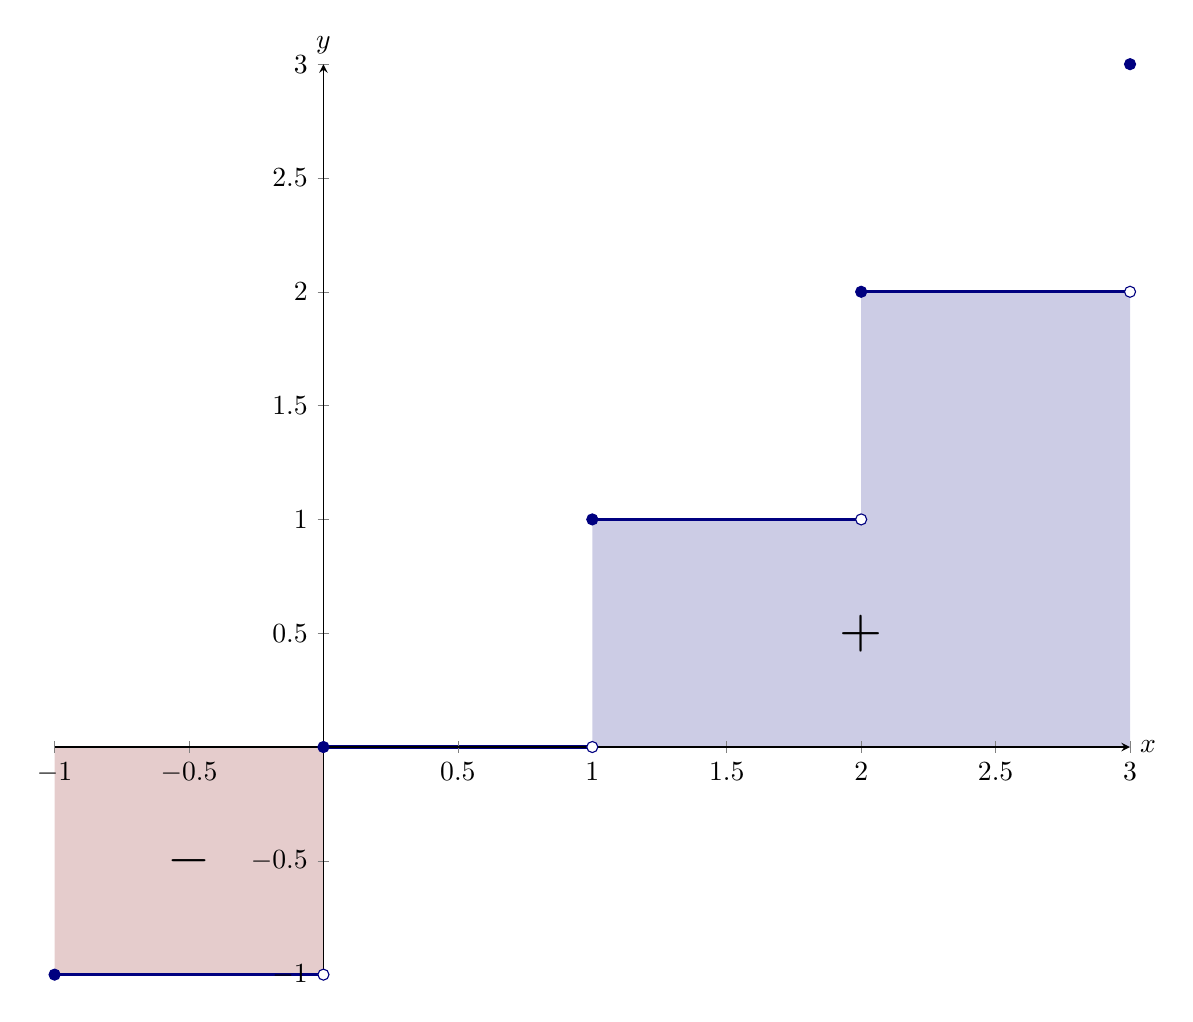
\begin{tikzpicture}
\colorlet{penColor}{blue!50!black}
\colorlet{fillp}{blue!50!black!20}
\colorlet{filln}{red!50!black!20}
\colorlet{textColor}{black}
\colorlet{background}{white}
  \begin{axis}[
      domain=-1:3,
      width=6in,
      axis lines =middle, xlabel=$x$, ylabel=$y$,
      every axis y label/.style={at=(current axis.above origin),anchor=south},
      every axis x label/.style={at=(current axis.right of origin),anchor=west},
      clip=false,
      axis on top,
    ]
    \addplot [draw=none, fill=filln, domain=(-1:0)] {-1} \closedcycle;
    \addplot [draw=none, fill=fillp, domain=(0:1)] {0} \closedcycle;
    \addplot [draw=none, fill=fillp, domain=(1:2)] {1} \closedcycle;
    \addplot [draw=none, fill=fillp, domain=(2:3)] {2} \closedcycle;
    \addplot [very thick, penColor, domain=(-1:0)] {-1};
    \addplot [very thick, penColor, domain=(0:1)] {0};
    \addplot [very thick, penColor, domain=(1:2)] {1};
    \addplot [very thick, penColor, domain=(2:3)] {2};
    \addplot[color=penColor,fill=penColor,only marks,mark=*] coordinates{(-1,-1)};  %% closed hole          
    \addplot[color=penColor,fill=penColor,only marks,mark=*] coordinates{(0,0)};  %% closed hole          
    \addplot[color=penColor,fill=penColor,only marks,mark=*] coordinates{(1,1)};  %% closed hole          
    \addplot[color=penColor,fill=penColor,only marks,mark=*] coordinates{(2,2)};  %% closed hole  
    \addplot[color=penColor,fill=penColor,only marks,mark=*] coordinates{(3,3)};  %% closed hole                  
    \addplot[color=penColor,fill=background,only marks,mark=*] coordinates{(0,-1)};  %% open hole
    \addplot[color=penColor,fill=background,only marks,mark=*] coordinates{(1,0)};  %% open hole
    \addplot[color=penColor,fill=background,only marks,mark=*] coordinates{(2,1)};  %% open hole
    \addplot[color=penColor,fill=background,only marks,mark=*] coordinates{(3,2)};  %% open hole

    \node at (axis cs:-.5,-.5) [textColor] {\scalebox{2}{$\boldsymbol-$}};
    \node at (axis cs:2,.5) [textColor] {\scalebox{2}{$\boldsymbol+$}};
  \end{axis}
\end{tikzpicture}

$\displaystyle\int_{-1}^3 \lfloor x \rfloor \d x =$ \answer{2}

\end{question}

\begin{question}
Use geometry to compute
\[
\int_{-5}^1 \sqrt{9-(x+2)^2}\d x.
\]
\begin{hint}
Plot the curve in question.
\end{hint}


$\displaystyle \int_{-5}^1 \sqrt{9-(x+2)^2}\d x$ = \answer{pi*81/2}
Express your answer in an exact form.
\end{question}

\begin{question}
Use geometry to compute
\[
\int_{1}^{-5} \sqrt{9-(x+2)^2}\d x.
\]
\begin{hint}
Plot the curve in question.
\end{hint}


$\displaystyle \int_{1}^{-5} \sqrt{9-(x+2)^2}\d x$ = \answer{-pi*81/2}
Express your answer in an exact form.
\end{question}




\begin{question}
Write down at least \textbf{five} questions for this lecture. After
you have your questions, label them as ``Level 1,'' ``Level 2,'' or ``Level 3'' where:
\begin{description}
\item[Level 1] Means you know the answer, or know exactly how to do this problem.
\item[Level 2] Means you think you know how to do the problem, or will soon learn how to do the problem.
\item[Level 3] Means you have no idea how to do the problem. 
\end{description}
  \begin{freeResponse}
  \end{freeResponse}
\end{question}

\end{document}
